\part{Lógica Computacional Árborea (CTL)}
\section{Sintaxis y semantica}
A diferencia de LTL, que se concentra en una única traza, nos va a permitir describir propiedades sobre la totalidad de las trazas de un sistema. Dejamos de verlas como caminos disconexos para pasar a representarlas como arboles de ejecución.

\begin{figure}[h]
\centering
	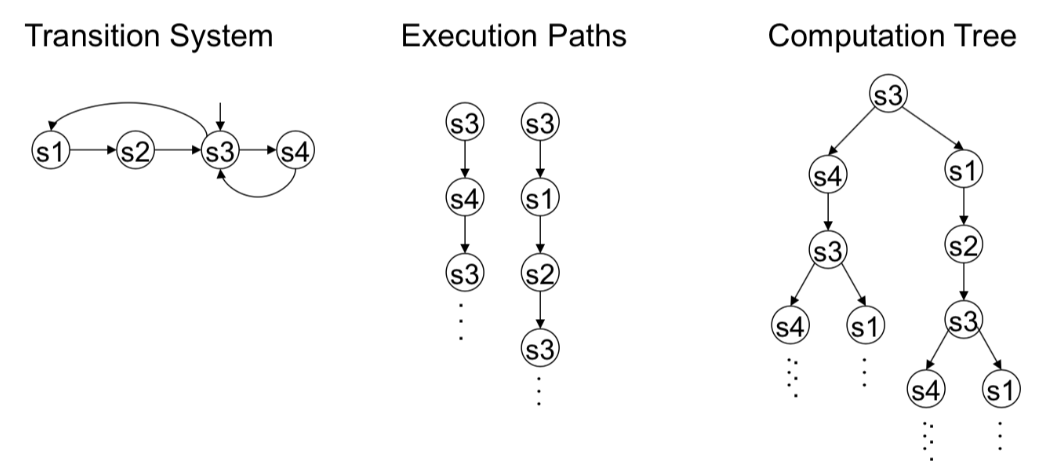
\includegraphics[scale=0.25]{imagenes/ctl-ltl-comparison}
\end{figure}

Agrega las cuantificaciones A y E a los operadores modales, lo que permite, asertar cosas sobre todos los caminos que derivan de un nodo:
\begin{itemize}
\item A: Para todo camino
\item E: Existe un camino
\end{itemize}

\begin{definicion}{Función de evaluación L}
Dado un conjunto de proposiciones atómicas $AP$ y una estructura de Kripke $M=(W,R)$ sobre $AP$, la función $L:W\to 2^{AP}$ toma un estado de $M$ y devuelve el conjunto de proposiciones que valen en ese estado (la imagen de la función es el conjunto de parte de AP).
\end{definicion}
\subsection{Semántica}
Dado un árbol de cómputo infinito satisface una formula si su raíz $s_0$ lo hace. Sean $\psi$ y $\psi_1$ dos fórmulas de CTL:
\begin{itemize}
    \item $s \vDash p$ si y solo si $v(p,s)$ (con $p$ una propoción atómica)
    \item $s_0 \vDash \text{EX } \psi$ si y solo si existe un camino $S =\{s_0,\dots\}$ tal que $S[1]\vDash \psi$
    \item $s_0 \vDash \text{AX } \psi$ si y solo si para todo camino $S$ de la forma $\{s_0,\dots\}$ vale que $S[1]\vDash \psi$
    \item $s_0 \vDash \text{EG } \psi$ si y solo si existe un camino $S =\{s_0,\dots\}$ en el que siempre vale $\psi$ .
    \item $s_0 \vDash \text{AG } \psi$ si y solo si para todo camino $S$ de la forma $\{s_0,\dots\}$ siempre vale $\psi$ ($\forall~i\geq 0$ vale $S[i] \vDash \psi$).
    \item $s_0 \vDash \text{EF } \psi$ si y solo si existe un camino $S=\{s_0,...\}$ en el que, en algún momento, vale $\psi$ ($\exists~i\geq 0$ tal que  $S[i] \vDash \psi$).
    \item $s[0] \vDash \text{AF } \psi$ si y solo si para todo camino  $S$ de la forma $\{s_0,\dots\}$ vale, en algún momento, $\psi$ ($\exists~i\geq 0$ tal que  $S[i] \vDash \psi$).
    \item $s_0 \vDash \psi \text{ EU } \psi_1$ si y solo si existe un camino $S =\{s_0,\dots\}$ tal que \\\hspace*{1cm} $(\exists i\geq 0)~(S[i] \vDash \psi_1~\land~(\forall~ 0\leq j\leq i)~S[j]\vDash \psi))$.
    \item $s_0 \vDash \psi \text{ AU } \psi_1$ si y solo si para todo camino  $S$ de la forma $\{s_0,\dots\}$ vale que\\\hspace*{1cm} $(\exists i\geq 0)~(S[i] \vDash \psi_1~\land~(\forall~ 0\leq j\leq i)~S[j]\vDash \psi))$.
\end{itemize}

\subsubsection{Equivalencias}\label{sec::ctlEquivalencias}
\begin{itemize}
\item AX $\psi~\equiv~\lnot$ EX $(\lnot \psi)$
\item AG $\psi~\equiv~\lnot$ EF($\lnot \psi$)
\item EF $\psi~\equiv$ ($true$ EU $\psi$)
\item AF $\psi~\equiv~\lnot$EG($\lnot \psi$)
\item $\psi$ AU $\psi_1~\equiv~$AF $\psi_1 \land \lnot(\lnot \psi_2$ EU $\lnot(\psi\lor\psi_2))$
\end{itemize}
\newpage
\section{Verificación explicita de propiedades}
Dado una estructura de Kripke, deseamos determinar si su árbol de cómputo cumple con una fórmula $\psi$ de CTL. Para esto, debemos representar las fórmulas como conjuntos de estados.

\subsection{Fórmulas como conjuntos característicos}\label{sec::conjuntoCaracteristicos}
\begin{definicion}{Conjunto característico}
Dados un modelo $M = \langle(W,R), v\rangle$ sobre un conjunto de proposiciones átomicas ($AP$) y una fórmula de CTL $\phi$. El conjunto característico $\charset{\phi}{M}$ de $\phi$ sobre $M$ es el conjunto de estados en los que $\phi$ es verdadera.
\end{definicion}

\paragraph{Semántica de CTL vista como conjuntos característicos}
\begin{itemize}
\item $\charset{a}{M} = \{s \in W ~|~ v(s,a) = \text{True} \}$ para $a\in AP$
\item $\charset{\lnot\psi}{M} = W - \charset{\psi}{M}$
\item $\charset{\psi_1\lor\psi_2}{M} = \charset{\psi_1}{M} \cup \charset{\psi_2}{M}$
\item $\charset{\psi_1\land\psi_2}{M} = \charset{\psi_1}{M} \cap \charset{\psi_2}{M}$
\item $\charset{\text{EX }\psi}{M} = \{s\in W~|~\exists~(s,t)\in R$ tal que $t\in\charset{\psi}{M}\}$
\item $\charset{\text{EG }\psi}{M} = \{s\in W~|$ existe un camino $S=\{s,\dots\}$ tal que para todo estado $S[i]$ con $i\geq 0$, $S[i]\in\charset{\psi}{M} \}$
%
%Es el mayor conjunto $T\subseteq W$ que satisface:
%\begin{enumerate}
%\item $T\subseteq\charset{\phi}{M}$ (\textit{son estados que satisfacen $\phi$}) y
%\item $s\in T \implies$ Post$(s)\cap T \neq\emptyset$ (\textit{si un estado de $T$ tiene un estado siguiente, entonces ese estado también está en $T$}).
%\end{enumerate}

\item $\charset{\psi \text{ EU }\psi_2}{M} = \{s\in W~|$ existe un camino $S=\{s,\dots\}$ tal que para algún estado $S[i]$ con $i\geq 0$, $S[i]\in\charset{\psi_2}{M}$ y para todo $k < i$, $S[k]\in\charset{\psi}{M} \}$
%
%Es el mínimo conjunto $T\subseteq W$ que satisface las siguientes fórmulas:
%\begin{enumerate}
%	\item $\charset{\psi_2}{M}\subseteq T$ (\textit{todos los estados que satisfacen $\phi_2$ están en $T$}) y
%	\item $(s\in\charset{\psi}{M}~\land$ Post$(s)\cap T \neq\emptyset) \implies s\in T$ (\textit{si un estado de $T$ tiene un estado anterior que satisface $\phi_1$ entonces, ese estado, está en $T$})
%\end{enumerate}
%\end{itemize}
%
%\red{El resto de las caracterizaciones faltan en la teóricas, pero acá van:}
%\begin{itemize}
%\item $\charset{\text{AX }\phi}{M} = \{s\in W~|~\forall~t\in$ Post($s$) tal que $t\in\charset{\phi}{M}\} = \{ s \in W~|~$ Post($s) \subseteq \charset{\phi}{M}\}$.
%\item $\charset{\text{AG }\phi}{M} = \{s\in W~|$ para todo camino $S=\{s,\dots\}$ vale que $\forall~i\geq 0,~S[i]\in\charset{\phi}{M} \}$
%
%Es el mayor conjunto $T\subseteq W$ que satisface $T \subseteq \{ s \in\charset{\phi}{M}~|$ Post$(s) \subseteq T \}$.
%
%\item $\charset{\phi_1 \text{ AU }\phi_2}{M} = \{s\in W~|$ para todo camino $S=\{s,\dots\}$ vale que para algún estado $S[i]$ con $i\geq 0$, $S[i]\in\charset{\phi_2}{M}$ y para todo $k < i$, $S[k]\in\charset{\phi_1}{M} \}$
%
%Es el mínimo conjunto $T\subseteq W$ que satisface 
%\begin{enumerate}
%\item $\charset{\phi_2}{M} \subseteq T$ y
%\item $\{s\in\charset{\phi_1}{M} ~|~$ Post$(s)\subseteq T\} \subseteq T$
%\end{enumerate}
\end{itemize}

Decimos que un modelo $M$ satisface $\psi$ ($M\vDash \psi$) si y solo si su estado inicial $s_0$  la satisface ($s_0 \in\charset{\psi}{M}$).

\newpage
\subsubsection{Algoritmo de verificación explícito:} 

\paragraph{Para EX $\psi$}: 
\begin{enumerate}
\item Conseguir todos los estados en los que vale $\psi$.
\item Hacer un paso hacia atrás en cada uno de ellos. (Todos estos conjuntos son los que cumplen la fórmula)
\end{enumerate}
\begin{figure}[h]
\centering
	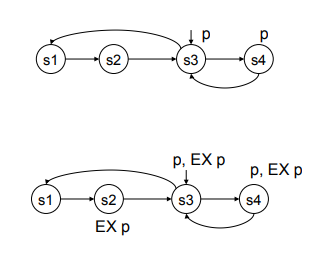
\includegraphics[scale=0.5]{imagenes/computo-ex-explicito}
	\caption{Cómputo de EX}
\end{figure}

\paragraph{Para $\psi$ EU $\psi_1$}: 
\begin{enumerate}
\item Conseguir todos los estados en los que vale $\psi_1$ (estos estados cumplen la fórmula)
\item Ir hacía atras mientras valga $\psi$ (cada estado por el que pasamos cumple la fórmula).
\end{enumerate}
\begin{figure}[h]
\centering
	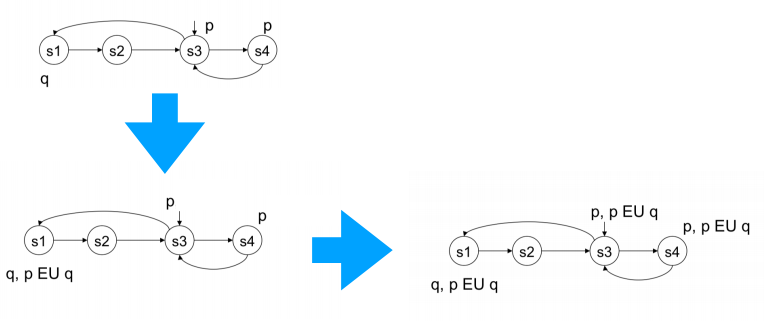
\includegraphics[scale=0.5]{imagenes/computo-eu-explicito}
	\caption{Cómputo de EU}
\end{figure}
\paragraph{Para EG $\psi$}: 
\begin{enumerate}
\item Eliminar todos los estados en donde no vale $\psi$ y conectar los nodos que quedan. Osea, que hay que remplazarlo por caminos entre cada uno de sus nodos de entrada a todos sus nodos de salida.
\item Computar las componentes fuertemente conexas.
\item Marcar todos los estados del Kripke en los que valen $p$ que llegan a alguna componente fuertemente conexa.
\end{enumerate}

\begin{figure}[h]
\centering
	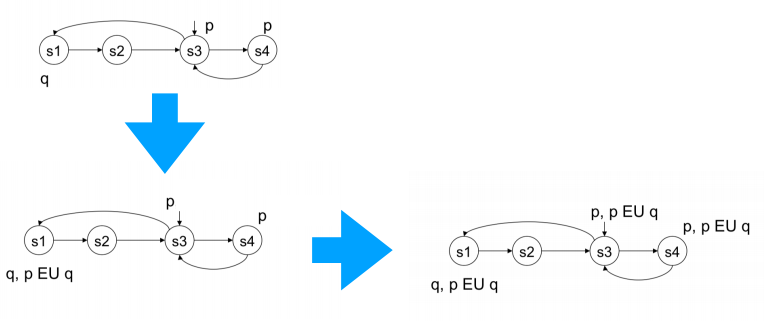
\includegraphics[scale=0.5]{imagenes/computo-eu-explicito}
	\caption{Cómputo de EG}
\end{figure}

\paragraph{Para el resto de las fórmulas:} Convertirlas a fórmulas que solo usen EX, EG y EU usando las equivalencias de la sección \ref{sec::ctlEquivalencias}. Y aplicar alguno de los algoritmos anteriores.

\newpage
\section{Verificación implícita de propiedades}
El algoritmo visto en la sección anterior, utiliza distintas técnicas para recorrer grafos, por lo que se necesita una representación explicita del espacio de estados del modelo. Esto limita los sitemas que podemos representar ya que, por ejemplo, en sistemas concurrentes la cantidad de estados aumenta exponencialmente con la cantidad de sub-procesos compuestos.

Por  esta razón, se desarrolló lo que se llama la verificación simbólica de propiedades. Esta técnica utiliza diagramas de binarios de decisión para representar el sistema como una fórmula proposicional lógica que podemos que conjugar con la propiedad que deseamos verificar.

La fórmula obtenida describe los estados del modelo en los que la propiedad vale.

\subsection{Arboles binarios de decision}
Si bien, las fórmulas booleanas/LTL que tratamos en clase no tienen muchas proposiciones y están bastante sintetizadas, en la vida real no es así. En muchos casos, tendremos demasiadas variables y no será fácil escribir una formula sintácticamente compactas, es decir, nos puede pasar que haya operaciones innecesarias. 

Resolver esta fórmula, implicaría evaluar toda las proposiciones que están en esta parte innecesaria, por lo menos, una vez y ocupar tiempo de computo en operaciones booleanas sin sentido. Si bien, evaluarla una vez, no parece que tenga mucho impacto, hacer esto para cada estado de un Kripke implicaría demasiado tiempo.

Pongamos un ejemplo: Si $a$ y $b$ son las variables proposicionales de nuestro modelo, sea $\psi = (\lnot a\land b) \lor (a\land b)$. Vemos que $(\lnot a\land b) \lor (a\land b)$ es equivalente a $b$. Osea que en cada estado que evaluemos $\psi$, estaríamos evaluando innecesariamente dos veces $a$ y a $b$ una vez de más.

\paragraph{Árboles de decisión binarios (BDT):} Son estructuras que pueden ser usados para representar y manipular fórmulas booleanas. La cantidad de nodos de un BDT es $2^n-1$, con $n$ la cantidad de variables proposicionales de la fórmula representada.
\begin{figure}[h]
\centering
	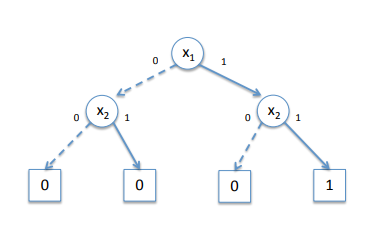
\includegraphics[scale=0.5]{imagenes/binary-decision-tree}
	\caption{Árbol de decisión binaria para $x_1 \land x_2$}
\end{figure}

\paragraph{Diagramas de decisión binaria (BDD):} Son una representación más compacta de los BDT. Eliminan la representación redundante de variables booleanas y permite compartir sub-árboles iguales.

Son representaciones canónicas, es decir, dada dos fórmulas semanticamente equivalentes, si damos un orden a sus variables y creamos sus BDD para cada una de ellas entonces, los BDD, serán iguales. Osea que, en el ejemplo anterior, $\psi$ y $b$ tienen el mismo árbol. De esta forma, evitamos  realizar evaluaciones de más.
\begin{figure}[h]
\centering
	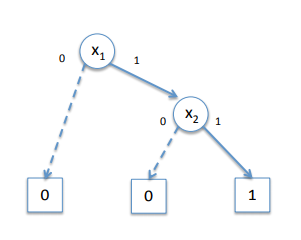
\includegraphics[scale=0.5]{imagenes/bdd}
	\caption{Diagrama de decisión binaria para $x_1 \land x_2$. El nodo $x_2$ del lado izquierdo era redundante porque la fórmula da siempre $0$ sin importar su valor.}
\end{figure}

\subsubsection{Construcción de un ROBDD}
Dada una fórmula queremos conseguir un OBDD reducido para la misma:
\begin{enumerate}
\item Dividir la fórmula en sub-formulas hasta llegar a las variables proposicionales.
\item Crear un ROBDD para cada proposición e ir combinandolos para obtener cada sub-fórmula. Luego, para cada ROBDD, crearlos e ir componiendolos hasta llegar a la fórmula
\end{enumerate}

\paragraph{Algoritmo de composición de ROBDD}:
Dados dos ROBDD $A$ y $B$ que representan las fórmulas $\phi$ y $\psi$,respectivamente que hayan sido creados con el mismo orden de variables:

\begin{enumerate}
\item Elegir un ROBDD por el que empezar y tomar la raíz.
\item Si la variable representada por la raíz no está en el otro OBDD entonces agregarla como raíz, con ambos caminos apuntando hacia la raíz original.
\item Elegir un camino y seguirlo hasta el próximo nivel en ambos ROBDD. Si los niveles no representan las mismas variables, entonces agregar un nodo hipotético entre ambos niveles. Ambos caminos del nodo hipotetico van al nivel más bajo.
\item Si llegamos a las hojas, conseguimos un valor para $phi$ y uno para $\psi$, aplicarles la operación lógica que queremos conseguir.
\item Agregar el camino recorrido (con los nodos hipotéticos) a un nuevo árbol y poniendo como hoja el resultado de la operación. Y eliminando ocurrencias redundantes (nodos cuyos caminos van al mismo nodo).
\item Volver a repetir para cada camino posible.
\end{enumerate} 



\paragraph{Ejemplo:} Queremos conseguir el ROBDD de $(x_1\lor x_2)\land(\lnot x_1\lor \lnot x_2)$, el árbol sintáctico de la fórmula es:

\begin{center}
	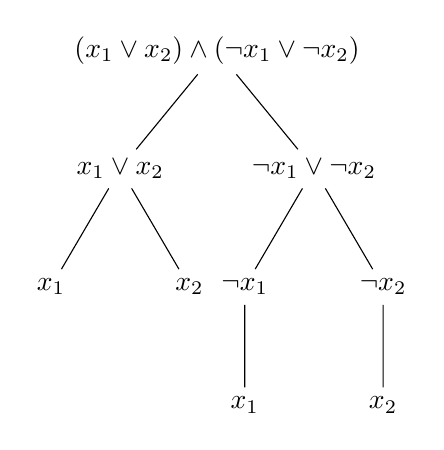
\begin{tikzpicture}[level 1/.style={sibling distance=7em},
	level 2/.style={sibling distance=5em}]
		\node {$(x_1\lor x_2)\land(\lnot x_1\lor \lnot x_2)$}
			child { node {$x_1\lor x_2$}
				child	{ node {\red{$x_1$}}}
				child { node {\red{$x_2$}}}
			}
			child { node {$\lnot x_1\lor \lnot x_2$}
				child{node {$\lnot x_1$}
					child{ node{\red{$x_1$}} }
				}
				child { node {$\lnot x_2$}
					child {node {\red{$x_2$}}}
				}
			}
		;
	\end{tikzpicture}
\end{center}

Osea que, para empezar, debemos construir los OBDDs para $x_1$ y $x_2$:
\begin{figure}[h]
\centering
	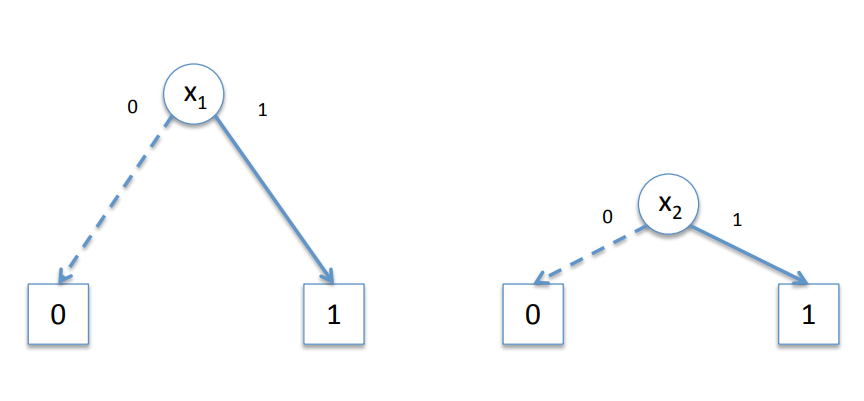
\includegraphics[scale=0.25]{imagenes/compo-obdd1}
\end{figure}

Para conseguir el OBDD de $x_1\lor x_2$, debemos recorrer los dos árboles asignando, en cada nivel, un valor a la variable de ese nivel. Empezamos por el de $x_1$. Como en el árbol de la derecha no existe, le agregamos un nodo hipotético como raíz.
\begin{center}
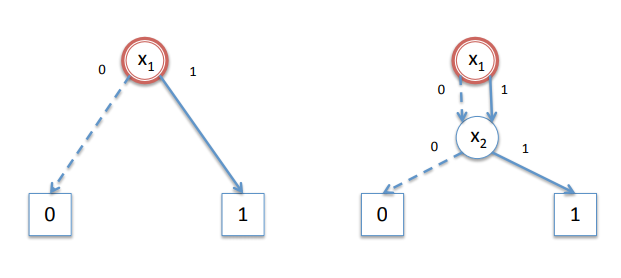
\includegraphics[scale=0.35]{imagenes/compo-bdd2}
\end{center}

Elegimos el camino $x_1 = 0$ y avanzamos al siguiente nivel que, en el lado derecho, corresponde a $x_2$ y falta en el izquierdo:
\begin{center}
	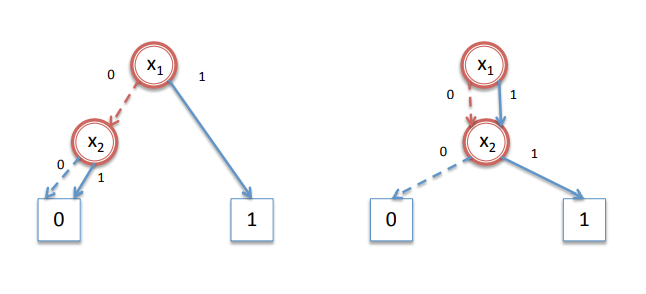
\includegraphics[scale=0.35]{imagenes/compo-obdd3}
\end{center}

Y elegimos el camino $x_2 = 0$:

\begin{center}
	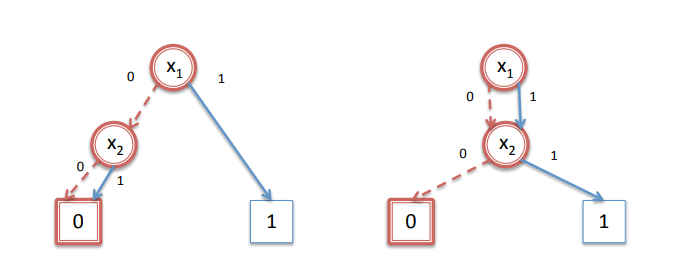
\includegraphics[scale=0.35]{imagenes/compo-robdd4}
\end{center}

Conseguimos el valor $0$ en ambos árboles. $0\lor0$ es $0$, entonces creamos un nuevo árbol con el cámino que acabamos de recorrer y el valor $0$ como hoja:
\begin{center}
	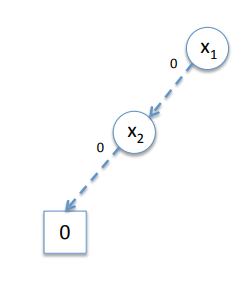
\includegraphics[scale=0.35]{imagenes/compo-robdd5}
\end{center}

Ahora, subimos un nivel, y elegimos $x_2 = 1$:

\begin{center}
	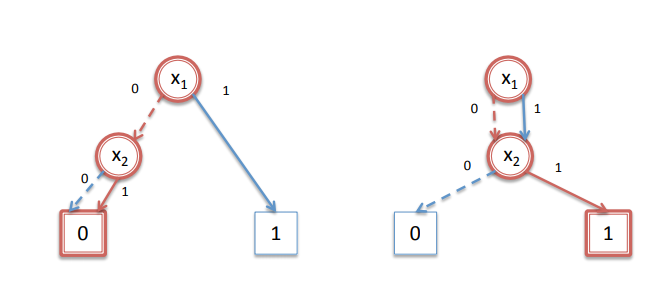
\includegraphics[scale=0.35]{imagenes/compo-robdd6}
\end{center}

Conseguimos los valores $0$ y $1$. Combinandolos con $\lor$ obtenemos $1$, entonces agregamos ese camino al árbol que estamos creando:

\begin{center}
	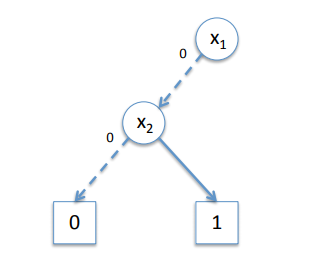
\includegraphics[scale=0.35]{imagenes/compo-robdd7}
\end{center}

Como ya consideramos todos los posibles valores de $x_2$ para cuando $x_1 = 0$, subimos dos niveles y vemos el caso $x_1 = 1$ y $x_2 = 0$:

\begin{center}
	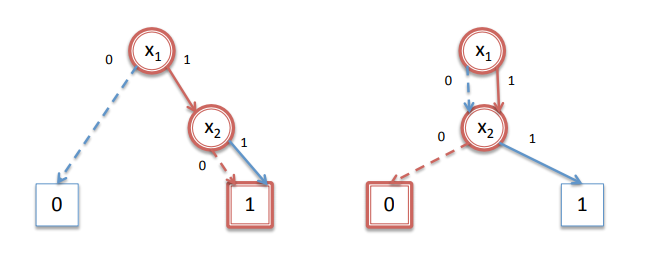
\includegraphics[scale=0.35]{imagenes/compo-robdd8}
\end{center}

Es el mismo caso que el anterior, agregar el camino y terminarlo en $1$:

\begin{center}
	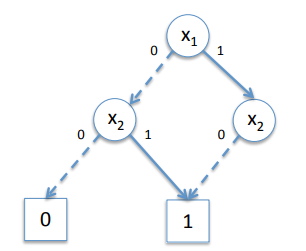
\includegraphics[scale=0.35]{imagenes/compo-robdd9}
\end{center}

Analizamos el único camino que falta ($x_1 = 1$ y $x_2 = 2$):
\begin{center}
	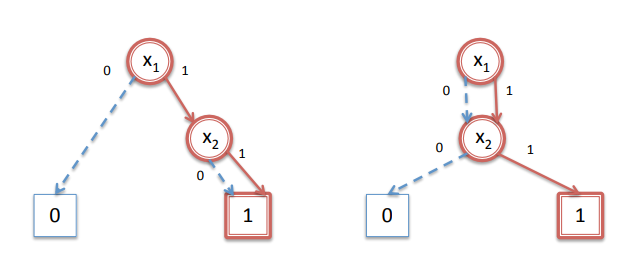
\includegraphics[scale=0.35]{imagenes/compo-robdd10}
\end{center}

Ambos valores son $1$ y $1\lor1 = 1$:
i\begin{center}
	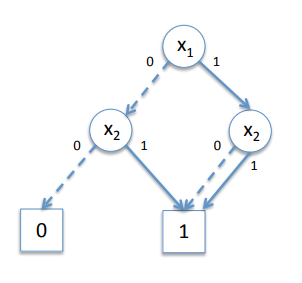
\includegraphics[scale=0.35]{imagenes/compo-robdd11}
\end{center}

Vemos que cuando $x_1 = 1$, el nodo de $x_2$ es redundante, pues ambos caminos van a $1$. Entonces, lo eliminamos:
\begin{center}
	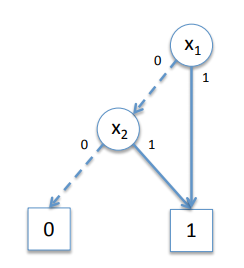
\includegraphics[scale=0.35]{imagenes/compo-robdd12}
\end{center}

Para crear los ROBDD para la negación, solo hay que invertir los valores de las hojas del ROBDD de la fórmula que queremos negar. Luego combinamos ambos ROBDDs de la misma forma para obtener $\lnot x_1 \lor \lnot x_2$

Por último, usando el mismo algoritmos, combinamos los ROBDDs de $\lnot x_1 \lor \lnot x_2$ y $x_1 \lor x_2$ para conseguir la fórmula original.


\subsection{Cálculo de EX $\psi$}
Ya sabemos como caracterizar los estados de un Kripke que cumplen con un fórmula CTL $\psi$ y, además tenemos una buena forma de representar y evaluar fórmulas booleanas (los OBDDs). Lo siguiente, será definir un algoritmo que nos permita encontrar una fórmula booleana que describa los estados que satisfacen $\psi$.

Dado un modelo $\mathcal{M} = \langle(W,R),v\rangle$ y una formula $\psi$, queremos obtener una fórmula que podamos evaluar en cada estado del Kripke que devuelva \textit{true} cuando ese estado cumple EX $\psi$.

Vamos a ir haciendolo con un ejemplo, supongamos que tenemos el siguiente Kripke cuyas propocisiones son $p$ y $q$:


\begin{center}
\begin{tikzpicture}[
	every state/.style={fill=black!10, align=center, minimum size=1.25cm},
	initial text=$ $,
	edge/.style = {-{Stealth}}
]
\node[state, initial] (s0) {0 \\ $\emptyset$};
\node[state] (s1) [below=of s0] {1 \\ $p$}; 
\node[state] (s2) [right=of s1]{2 \\ $p,q$}; 
\node[state] (s3) [above=of s2]{3 \\$q$};

\draw[edge] (s1.10) to (s2.170);
\draw[edge] (s2.190) to (s1.-10);
\draw[edge] (s0.10) to (s3.170);
\draw[edge] (s3.190) to (s0.-10);

\draw[edge] (s0.280) to (s1.80);
\draw[edge] (s1.100) to (s0.260);
\draw[edge] (s3.280) to (s2.80);
\draw[edge] (s2.100) to (s3.260);

\end{tikzpicture}
\end{center}

\subsubsection{Conversión de un Kripke a fórmulas booleanas}
Una forma de describir un Kripke, es usando un estado inicial y un conjunto de transiciones. Si logramos representar cada uno de ellos como una fórmula booleana, ganamos.
\begin{enumerate}
\item Describir el estado inicial como una fórmula booleana \textit{I}. Esto es fácil, a cada estado inicial lo podemos representar como la conjunción de todas las variables proposicionales que valen en ese estado con la negación de todas las que no valen.

Si hay más de un estado inicial, se hace la disyunción de todas sus fórmulas.

\begin{center}
\begin{minipage}{0.8\textwidth}
En nuestro caso, solo tenemos un estado inicial en el que no vale ninguna de las propocisiones del modelo, entonces $I = \lnot q \land \lnot p$.
\end{minipage}
\end{center}

\item Describir las transición del Kripke como una fórmula booleana $R$. Para esto, necesitamos hacer una conyunción de las fórmulas de cada transición.

La fórmula de una transición debe describir el estado actual de las variables y el estado que tendrá en el próximo paso. Para indicar el segundo caso, primamos las variables, es decir, les agregamos un apostrofe.

\begin{center}
\begin{minipage}{0.8\textwidth}
Nombro $R_{ij}$ a la transición que va de el estado $i$ al $j$, entonces tenemos:
\begin{multicols}{2}
\begin{itemize}
\item[] $R_{01} = \lnot p \land\lnot q \land \lnot q' \land p'$
\item[] $R_{03} = \lnot p \land\lnot q \land q' \land \lnot p'$
\item[] $R_{10} = p \land\lnot q \land \lnot q' \land \lnot p'$
\item[] $R_{12} = p \land\lnot q \land q' \land p'$
\item[] $R_{21} = p \land q \land \lnot q' \land p'$
\item[] $R_{23} = p \land q \land q' \land \lnot p'$
\item[] $R_{30} = \lnot p \land q \land \lnot q' \land \lnot p'$
\item[] $R_{32} = \lnot p \land q \land q' \land p'$
\end{itemize}
\end{multicols}
$$R = R_{01} \lor R_{03} \lor R_{10} \lor R_{12} \lor R_{21} \lor R_{23}\lor R_{30} \lor R_{32}$$
\end{minipage}
\end{center}
\end{enumerate}

Con $I$ y $R$ nos alcanza para describir el Kripke $K = I \land R$.

\subsubsection{Eliminación del existencial}
En la sección \ref{sec::conjuntoCaracteristicos}, vimos que EX $\psi$ es el conjunto de estados $\{s\in W~|~\exists~(s,t)\in R \land t\in\charset{\psi}{M}\}$. Tenemos que pensarlo como fórmula booleana que describa estados del Kripke.

$$\text{EX} \psi \equiv \exists V' \cdot R \land \psi[V' / V]$$

Esto es, si aplicamos EX $\psi$ a un estado, entonces ese estado lo cumple si existe un conjunto $V'$ de variables proposicionales tal que vale $R$ (hay una transición desde ese estado al nuevo) y $\psi[V' / V]$ (si remplazamos las variables proposicionales de $V$ por sus primadas, entonces vale $\psi$). El $\exists V'$ se traduce en un existencial por cada variable del conjunto de propocisiones.

Seguimos sin tener una fórmula proposicional, debemos eliminar el existencial, para esto hay que aplicar la siguiente equivalencia. Si $f$ y $v$ una proposición:

$$\exists v \cdot f = f[True/v] \lor f[False/v]$$


\paragraph{Seguimos con el ejemplo:} Supongamos que $\psi = p \land q$, queremos computar EX $\psi$.


\begin{align*}
\text{EX } \psi = &\exists V' \cdot R \land \psi[V' / V] \\
= &\exists V' \cdot R \land (p' \land q') \\
= &\exists p'\cdot(\exists q' \cdot R \land (p' \land q')) \\
= &\exists p'\cdot(R \land (p' \land q'))[\True/q'] \lor (R \land (p' \land q'))[\False/q'] \\
= &\exists p'\cdot(R[\True/q'] \land (p' \land q')[\True/q']) \lor (R[\False/q'] \land (p' \land q')[\False/q']) \\
= &\exists p'\cdot(R[\True/q'] \land (\underbrace{p' \land \True)}_{p'}) \lor \underbrace{(R[\False/q'] \land \underbrace{(p' \land \False)}_{\False})}_{\False} \\ 
= &\exists p'\cdot(R[\True/q'] \land p') \\
= &(R[\True/q'] \land p')[\True/p'] \lor (R[\True/q'] \land p')[\False/p']\\
= &(R[\True/q'][\True/p']  \land p'[\True/p'] )\lor (R[\True/q'][\False/p'] \land p'[\False/p'])\\
= &(R[\True/q'][\True/p']  \land \True) \lor (R[\True/q'][\False/p'] \land \False)\\
= & R[\True/q'][\True/p']\\
= &(R_{01} \lor R_{03} \lor R_{10} \lor R_{12} \lor R_{21} \lor R_{23}\lor R_{30} \lor R_{32})[\True/q'][\True/p'] \\
= &(\underbrace{R_{01}[\True/q'] }_{\False}\lor R_{03}[\True/q'] \lor \underbrace{R_{10}[\True/q']}_{\False} \lor R_{12}[\True/q']\\ & \lor \underbrace{R_{21}[\True/q'] }_{\False}\lor R_{23}[\True/q']\lor \underbrace{R_{30}[\True/q']}_{\False} \lor R_{32}[\True/q'])[\True/p'] \\
= &((R_{03}[\True/q'] \lor R_{12}[\True/q'] \lor R_{23}[\True/q'] \lor R_{32}[\True/q'])[\True/p'] \\
= &\underbrace{R_{03}[\True/q'][\True/p']}_{\False}  \lor R_{12}[\True/q'][\True/p']  \lor \underbrace{R_{23}[\True/q'][\True/p']}_{\False}   \\ &\lor R_{32}[\True/q'][\True/p'] \\
= & R_{12}[\True/q'][\True/p'] \lor R_{32}[\True/q'][\True/p'] \\ 
=& (p \land\lnot q \land q' \land p')[True/q'][True/p'] \lor (\lnot p \land q \land q' \land p')[True/q'][True/p'] \\
=& (p \land\lnot q \land True \land True) \lor (\lnot p \land q \land True \land True)\\
=& (p \land\lnot q) \lor (\lnot p \land q )\\
\end{align*}

Entonces $(p \land\lnot q) \lor (\lnot p \land q )$ describe los estados de este autómata que satisfacen la fórmula EX $\psi$. 

\subsection{Algoritmo de punto fijo}
Al resto de las fórmulas, las describimos de manera recursiva con EX y AX. Esto nos va a permitir utilizar los algoritmos de punto fijo para calcular los conjuntos de estados que satisfagan ciertas fórmulas.

\subsubsection{Los puntos fijos de un reticulado}
\begin{definicion}{Punto fijo}
Dada una función $f:D\to D$, $x\in D$ es un punto fijo de $f$, si y solo sí $f(x)=x$
\end{definicion}

\begin{definicion}{Función monótona}
Una función $f:D\to D$ es monótona si y solo si para todo $x,y\in D$, $x\leq y \implies f(x) \leq f(y)$
\end{definicion}


\begin{definicion}{Reticulado}
Un reticulado es un conjunto $S$ con una relación binaria $\mathcal{R}\subseteq S\times S$ (reflexiva, transitiva y antisimétrica) que define un orden parcial sobre sus elementos.

La relación, además, define un único \textbf{supremo} y un único \textbf{ínfimo} para cada par $(a,b)\in R$, es decir, vale que $a > b$ ó $b < a$.

En ingeniería notamos $a\lor b$ al supremo entre ambos valores y $a \land b$ al ínfimo.
\end{definicion}

\begin{definicion}{Reticulado completo}
Un reticulado es completo si cumple que para todo subconjunto de $S$ existe un supremo y un ínfimo.
\end{definicion}

En nuestro caso, los operadores de ínfimo y supremos van a estar dados por la intersección y la unión, respectivamente.

Por ejemplo, dado un conjunto de partes $P$, podemos definir su supremo como $ \bigcup\{ s | s \in P\} = P$ y su ínfimo como $\bigcap\{s | s \in P\} = \emptyset$.

Para mostrar los siguientes teoremas vamos a asumir que $D$ es un conjunto de partes.

\paragraph{Teorema 1:} Dado un reticulado completo $(D, \subseteq)$ y una función $f:D\to D$ monótona, entonces su mínimo punto fijo es $\bigcap\{ y | f(y) \subseteq y\}$

\red{Notar que estamos definiendo $f$ como una función monótona sobre conjuntos. En la definición de más arriba, habría que cambiar $\leq$ por $\subseteq$}

%\paragraph{Demostración:} Primero tenemos que ver que el conjunto $z = \bigcap\{ y | f(y) \subseteq y\}$ es punto fijo. Para esto tenemos que ver que $f(z) \subseteq z$ y que $f(z)\supseteq z$.
%\begin{enumerate}
%\item[$\subseteq)$] Sea $x\in D$ tal que $f(x) \subseteq x$, entonces:
%\begin{enumerate}
%\item $x \in \{ y | f(y) \subseteq y\}$. Y como $z$ resulta de la intersección de $x$ con otros conjuntos que cumplen lo mismo, vale que $z\subseteq x$.
%\item  Además, como $f$ es monótona, $f(z) \subseteq f(x)$. Por lo que  $f(z) \subseteq f(x) \subseteq x$.
%\item Como agarramos un elementos cualquiera del conjunto  $\{ y | f(y) \subseteq y\}$, lo que dijimos vale para cualquier elementos del mismo. Osea que $\forall~x\in \{ y | f(y) \subseteq y\}$ vale que $F(z)\subseteq x$. Luego $F(z) \subseteq \bigcap \{ y | f(y) \subseteq y\} = z$.
%\end{enumerate} 
%
%\item[$\supseteq)$] Como $f(z) \subseteq z$ (por el paso anterior) y $f$ es monótona, tenemos $f(f(z)) \subseteq f(z)$. 
%\begin{itemize}
%\item Entonces, $f(z) \in \{ y | f(y) \subseteq y\}$.
%\item Además, como dijimos en $(c)$, $z$ es subconjunto de todos los elementos de $f(z) \in \{ y | f(y) \subseteq y\}$. Osea que, particularmente, es subconjunto de $f(z)$. Luego $z\subseteq f(z)$.
%\end{itemize}
%\end{enumerate}
%
%Logramos mostrar que $f(z)\subseteq z$ y $z \subseteq f(z)$, entonces $f(z) = z$. Ahora falta demostrar que es un ínfimo, es decir que todos los otros puntos fijos de $f$ contienen a $z$
%\begin{itemize}
%\item Sea $x\in D$ tal que $f(x) = x$, entonces $f(x) \subseteq x$.
%\item Luego, $x$ es un elemento del conjunto $\{ y | f(y) \subseteq y\}$, luego $z \subseteq x$
%\end{itemize}

\begin{definicion}{Función $\cup$-continua}
Una función monótona $f:D\to D$ con $D$ finito es $\cup$-continua si dado un conjunto de conjuntos que cumples $p_1\subseteq p_2\subseteq\dots$ implica que $f(\bigcup_i p_i) = \bigcup f(p_i)$
\end{definicion}

\paragraph{Teorema 2:} Dado un reticulado completo $(D,\subseteq)$ y una función monótona $\cup$-continua \\ $f:D\to D$ entonces el límite de la secuencia $\bigcup_i f^i(\emptyset) = f(\emptyset)\cup f(f(\emptyset)) \cup f(f(f(\emptyset)))\cup\dots$ es el mínimo punto fijo.

\paragraph{Teorema 3:} Dado un reticulado completo $(D,\subseteq)$ y una función monótona \\ $f:D\to D$ entonces existe un $j$ tal que $F^j(\emptyset) = F^{j+1}(\emptyset)$ y $F^j(\emptyset)$ es el mínimo punto fijo.

\paragraph{Teorema 4:} Dado un reticulado completo $(D,\subseteq)$ y una función monótona  $f:D\to D$ entonces el límite de la secuencia$\bigcap_i f^i(S) = f(S)\cup f(f(S)) \cup f(f(f(S)))\cup\dots$ es el máximo punto fijo.

\subsubsection{Operadores CTL definidos recursivamente}\label{sub::puntoFijoRecursivo}
\begin{multicols}{2}
\begin{itemize}

\item AG $p$ = $p~\land$ AX AG $p$
\item EG $p$ = $p~\land$ EX EG $p$
\item AF $p$ = $p~\lor$  AX AF $p$
\item EF $p$ = $p~\lor$  EX EF $p$
\item $p$ AU $q$ = $q~\lor$ ($p~\land$ AX ($p$ AU $q$))
\item $p$ EU $q$ = $q~\lor$ ($p~\land$ EX ($p$ AU $q$))

\item $\charset{\text{AG } p}{} =\charset{p}{}~\cap~\charset{\text{AX AG }p}{}$
\item $\charset{\text{EG } p}{} =\charset{p}{}~\cap~\charset{\text{EX EG }p}{}$
\item $\charset{\text{AF } p}{} =\charset{p}{}~\cup~\charset{\text{AX AF }p}{}$
\item $\charset{\text{EF } p}{} =\charset{p}{}~\cup~\charset{\text{EX EF }p}{}$
\item $\charset{p\text{ AU } q}{} =\charset{q}{} \cup (\charset{p}{}~\cap~\charset{AX(p\text{ AU } q)}{})$
\item $\charset{p\text{ EU } q}{} =\charset{q}{} \cup (\charset{p}{}~\cap~\charset{EX(p\text{ EU } q)}{})$

\end{itemize}

\end{multicols}

\subsubsection{Operadores CTL como puntos fijos}
Dado un modelo $M=\langle(S,R), L\rangle$, definimos las funciones $\cdot:2^S\to 2^S$ que dado un conjunto del conjunto de partes de $S$, nos devuelve los estados de ese conjunto que satisfacen la fórmula. 

Notación usada en la clase: $$\underbrace{\text{AF } p}_{\ref{nombre}} = \overbrace{\lambda y.}^{\ref{parametro}} \underbrace{p}_{\ref{satisfaceP}}\overbrace{\lor }^{\ref{operacion}}\underbrace{\text{AX } y}_{\ref{llamada}}$$


\begin{enumerate}[label={(}\arabic*{)}]
\item\label{nombre} Nombre de la función, dada una fórmula $p$, vamos a crear una para cada operador CTL.
\item\label{parametro} El parámetro de la función $y$ es un conjunto de estados. 
\item\label{satisfaceP} Es el subconjunto de estados de $y$ que satisfacen $p$. 
\item\label{operacion} Es una operación sobre conjuntos: $\lor$ es la unión y $\land$ es la intersección. 
\item\label{llamada} Son los estados de $S$ que cumplen AX $y$ ó EX $y$, osea que:
\begin{itemize}
\item AX $y$ son todos los estados de $S$ tal que todas sus transiciones van a algún estado de $y$.
\item EX $y$ son todos los estados de $S$ tal que alguna de sus transiciones va a algún estado de $y$.
\end{itemize}
\end{enumerate}

\paragraph{Funciones para punto fijo:}
\begin{itemize}
\begin{multicols}{2}
\item[] \textbf{Punto fijo mínimo}
\begin{itemize}
\item AF $p : \lambda y.~p~\lor$ AX $y$
\item EF $p : \lambda y. ~p~\lor$ EX $y$
\item $p$ AU $q: \lambda y.~ q \lor (p~\land$ AX $y$)
\item $p$ EU $q: \lambda y.~ q \lor (p~\land$ EX $y$)
\end{itemize}
\columnbreak
\item[] \textbf{Punto fijo máximo}
\begin{itemize}
\item $p$ AG $p: \lambda y. p \land$ AX $y$
\item $p$ AG $p: \lambda y. p \land$ AX $y$
\end{itemize}
\vfill\null
\end{multicols}
\end{itemize}

Siguiendo la idea de los teoremas de más arriba, para conseguir un punto fijo mínimo, debemos aplicar, iterativamente, la función al conjunto vacío hasta que se estabilize la solución.
\begin{algorithmic}
\State{$x \leftarrow False$}
\While {$x \neq f(x)$}
    \State $x \leftarrow f(x)$
\EndWhile
\end{algorithmic}
Para los puntos fijos máximos, hacemos exactamente lo mismpo pero, en vez de partir desde el conjunto vacío, partimos desde $S$ (el conjunto de todos los estados).